\begin{center}
  {\huge \bfseries 線形代数学テキスト\par \vspace{2mm}}
  {\large \bfseries --前後期統合とその先へ--\par}
\begin{large}
  \vspace{40mm}
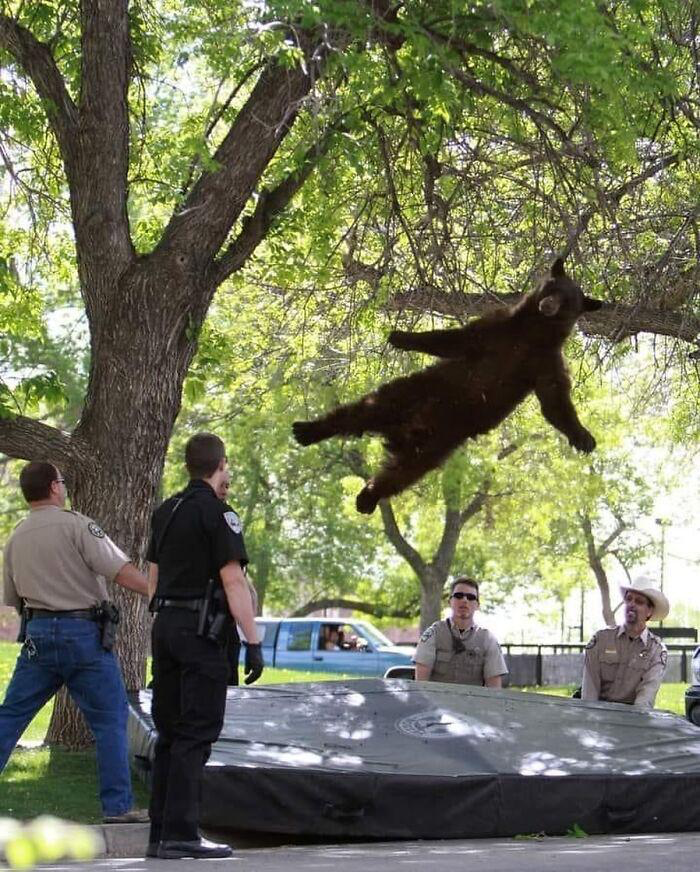
\includegraphics[width=0.6\hsize]{Welcome.png}
  \vspace{30mm}\par
  \underline{\hspace{1cm}著：関口 陽太\hspace{1cm}}
\end{large}
  \end{center}
\thispagestyle{empty}
\setcounter{page}{1}
\newpage
\begin{center}
    \textbf{概要}
\end{center}

まず,主張しておきたい.このテキストは\textbf{本大学の情報科学科に準拠した専用テキストである.}もちろん,年度が変われば,試験範囲に対応しきれなくなりうる.しかし,市販のテキストに比べれば最適化されていると考える.
「前期テキスト」「後期テキスト」と執筆してきましたが,今回これらの内容を統合しました.前期のテキストにおいては初めての作成もあって,見づらいところが散見されました.そこで,今回統合するにあたり,デザインの見直しを行いました.
また,線形代数学は単なる履修科目の枠組みを超え,他の専門科目において数学のツールとして使用していくことになります.これらの内容の説明を載せることで,今後の活用していけるのではないかと考え,新たに内容を追加しました.
\begin{center}
    テキストの流れ
\end{center}
\hspace{1em}
24年「線形代数学」の1Q,2Q,...の順番に試験範囲を完全カバーしつつ,関連する内容を追加しています.
試験範囲のみを優先して学習したい方もいらっしゃると思いますので,セクション名でわかるようにしました.
\begin{itemize}
  \item (重要)：試験範囲で必ず抑えたい内容
  \item 無記名：(重要)内容を説明するパート.暗記で乗り越える人には不要
  \item (発展)：試験範囲に関する発展的内容.範囲外だが,著者が紹介したい内容を掲載
  \item (科目名)：専門科目で使用する線形代数学の知識を掲載
\end{itemize}
\begin{center}
    内容の厳密性について
\end{center}

このテキストは数学科向けには作られていません.手段として線形代数学を使うに際し,証明や厳密な定義の理解,そ
れに対して注意を払うような行為はしないでしょう.理解のために証明を書くことはありますが,理解のための説明は
厳密性がなく,なんなら間違っている可能性もあるので,それによる事故は読者責任でお願いします.そして,私が判
断した内容や断言した内容はこのレベルでの線形代数学でのみ適用されて,もっと高度になると成り立たないという可
能性があることを十分に留意してほしい.しかし,最終的な結果 (公式) は間違っていないないようにはしています.
過去問で自分で色々テストしてみてください.
\begin{center}
    このテキストを使うにあたるルールと注意 (更新)
\end{center}
\begin{itemize}
    \item 外部への共有や公開の禁止
    \item 参考文献としての使用,記載禁止
    \item このテキストは購入者のみが使うことを想定しています.多少のグループでの共有は問題ないですが,
    その配慮はこのテキストが有料であることを考えての範囲にとどめてください.
\end{itemize}
\newpage
\begin{figure}[H]
\centering
  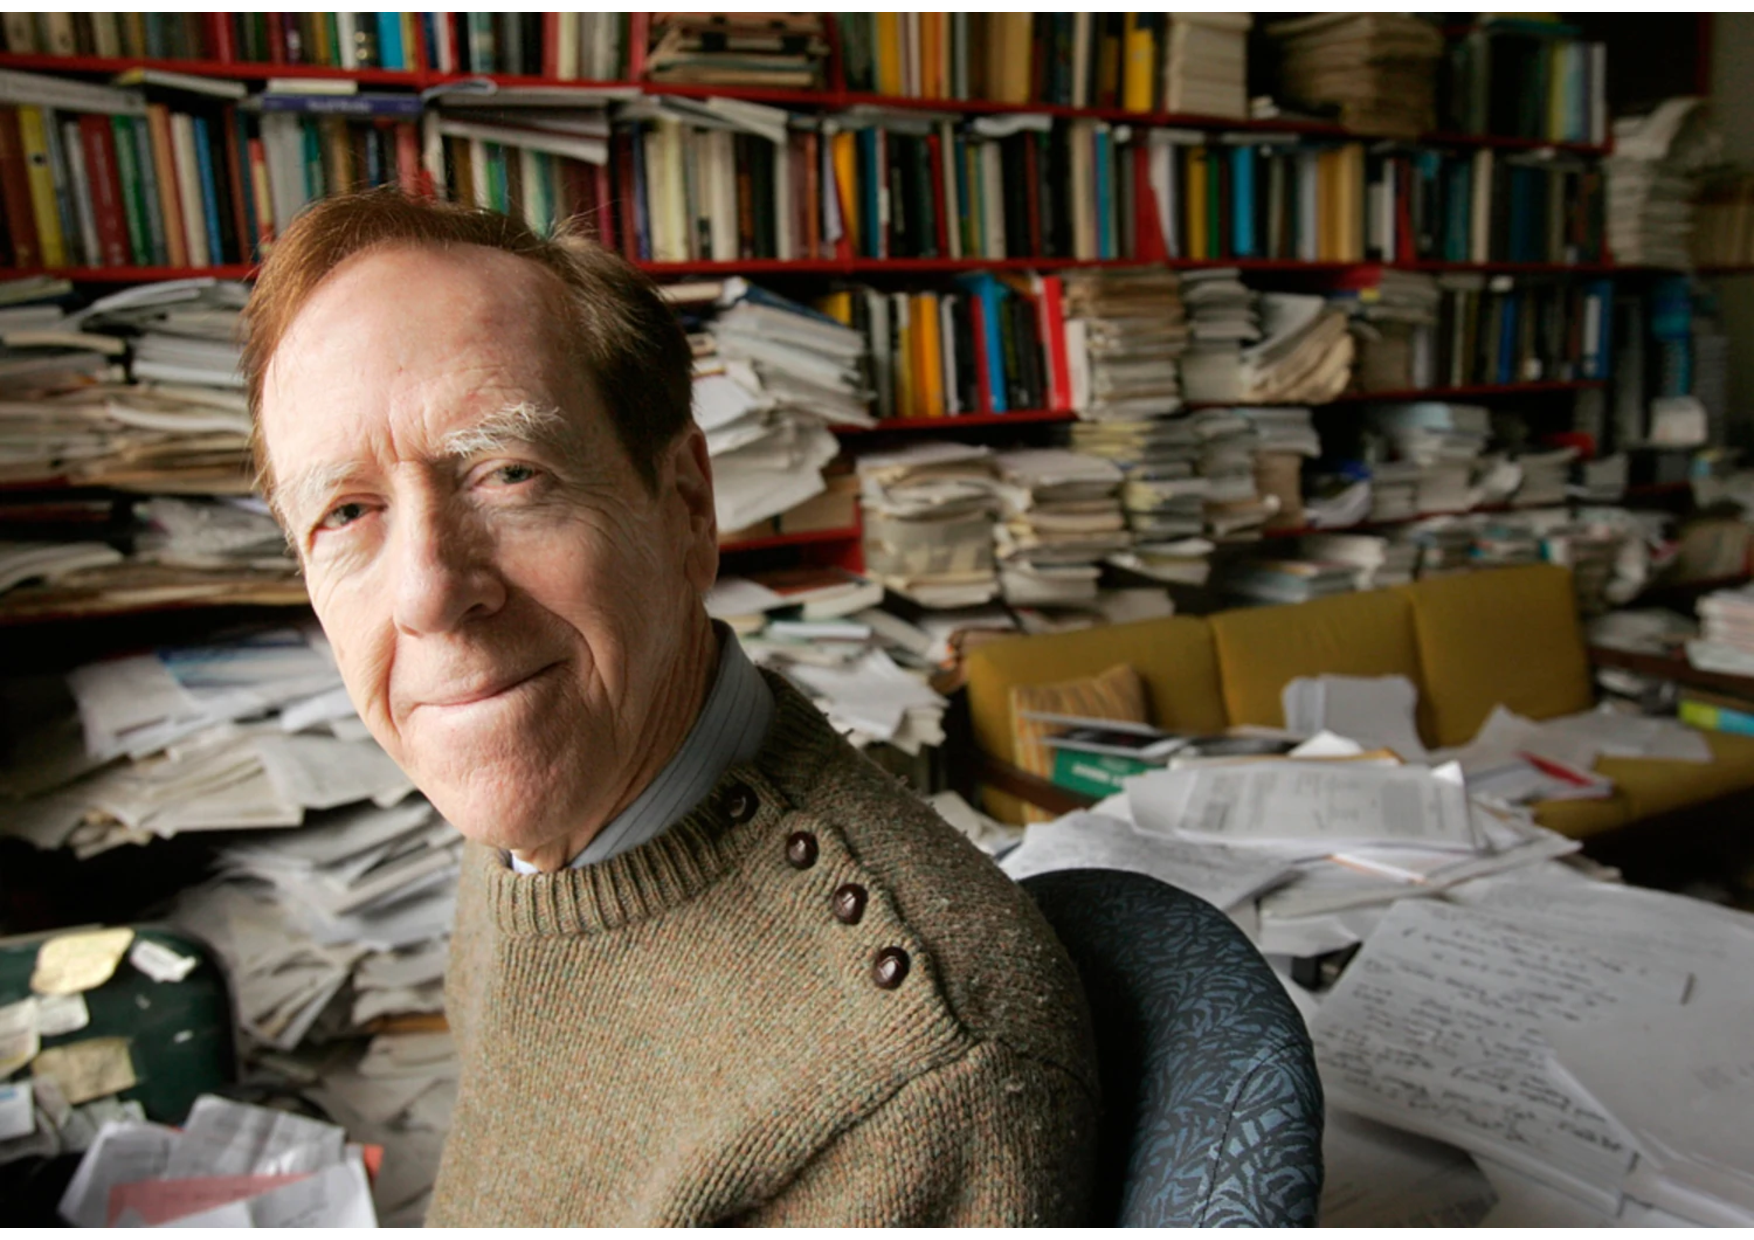
\includegraphics[width=0.5\hsize]{strang.pdf}
  \caption{Gilbert Strang先生}
  \label{fig:strang}
\end{figure}
\textbf{-著者について-}

24年入学.線形代数学(1a),(1b)は「良」だったが,大学では線形代数学が必要だというChatGPTの言葉を信じて1年終わりに独学で学習を始める.手に取ったストラング(図\ref{fig:strang})の本$^{\cite{strang}}$がとてもおもしろく,線形代数学の面白さを共有したいと同時に,まとめることで自身の知識の整理になると考えテキストの執筆を開始.

図\ref{guitar}は自慢のギター.B'zファンでシグネチャーモデルを購入して演奏していた.執筆時(2025年)しばらく触ってなかったが再び弾き始めよう画策していた.

図\ref{scean}は同年夏休みに行った,大阪万博旅行時の写真.旅仲間は2024年線形1a解答解説の監査メンバー.
\begin{minipage}[l]{0.49\textwidth}
\begin{figure}[H]\centering
  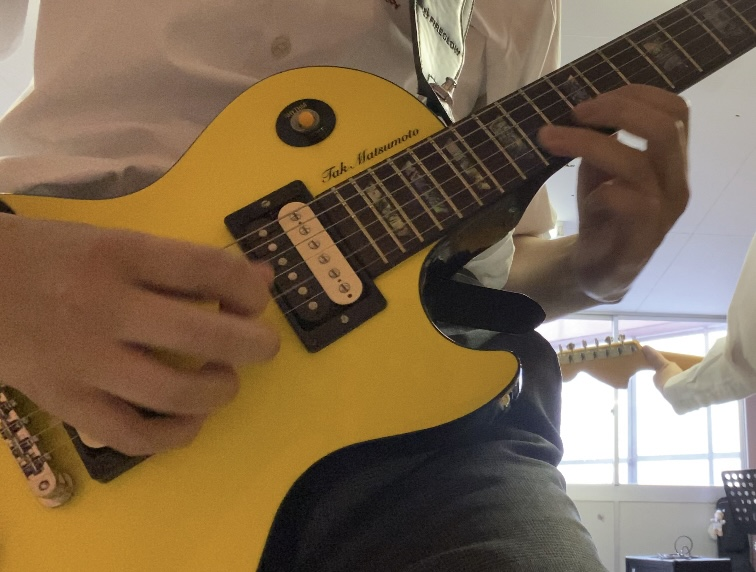
\includegraphics[width=0.7\hsize]{guitar.jpg}
  \caption{キャナリーイエロー}
  \label{guitar}
\end{figure}
\end{minipage}
\hfill
\begin{minipage}[l]{0.49\textwidth}
\begin{figure}[H]\centering
  \includegraphics[width=0.5\hsize]{scene .pdf}
  \caption{京都の一幕}
  \label{scean}
\end{figure}
\end{minipage}
\newpage
\tableofcontents
\newpage
